\documentclass[a4paper, 12pt]{article}
\usepackage[german]{babel} % deutsch, deutsche Rechtschreibung
\usepackage[utf8]{inputenc} % Unicode-Zeichensatz als Text-Quelle
\usepackage[T1]{fontenc} % Umlaute und deutsches Trennen
\usepackage{mathptmx} % Times New Roman, gewohnter Font
%\usepackage{uarial} % Setzt den gesamten Text in Arial
\usepackage{courier} % einen schickeren Schreibmaschinenfont
\usepackage[scaled=.95]{helvet} % was serifenloses, wenn gebraucht
\usepackage{graphicx} % wir wollen Bilder einfügen
\usepackage{xfrac} % schöne Brüche im Fließtext mit sfrac

\usepackage{hyperref}
  
\usepackage{listings} % Schöne Quellcode-Listings [minted wäre besser]


\lstset{basicstyle=\sffamily, columns=[l]flexible, mathescape=true, 
  showstringspaces=false, numbers=left, numberstyle=\tiny}
\lstset{language=python} % und nur schöne Programmiersprachen ;-)
% und eine eigene Umgebung für Listings

\usepackage{float} % eigene Fließobjekte, kommen an beliebigen Stellen vor
\newfloat{listing}{htbp}{scl}[section] % Nummeriere je Abschnitt
\floatname{listing}{Listing} % listing ist ein Fließobjekt

% Auch wenn es anrüchig ist, man kann den Platz etwas mehr ausnützen
\usepackage[paper=a4paper,width=15cm,left=35mm,height=22cm]{geometry}
\usepackage{setspace}
\linespread{1.2} % nicht ganz anderthalbzeilig, nur ein bisschen mehr Platz - war 1.15
\setlength{\parskip}{0.4em} % kleiner Paragraphen(Absatz)-abstand
\setlength{\parindent}{0em} % im Deutschen Einrückung nicht üblich

% Seitenmarkierungen 
\usepackage{fancyhdr} % Schickere Header und Footer
\pagestyle{fancy}
% Zeichensatz für Header/Footer
\newcommand{\phv}{\fontfamily{phv}\fontseries{m}\fontsize{9}{11}\selectfont}
\fancyhead[L]{\phv \leftmark} % Kurztitel links oben
\fancyhead[R]{\phv \thepage} % rechts oben die Seitenzahl
\fancyfoot[L]{\phv Hochschule Mannheim} % Institution links unten
\fancyfoot[C]{\ } % keine Seitenzahl unten Mitte
\fancyfoot[R]{\phv Medizintechnik} % Studiengang rechts unten

\usepackage{url} % wir wollen eine URL anzeigen



\begin{document}

\begin{titlepage}
	\centering
	%\vspace*{2cm} %Abstand nach oben

	% Logos:	
    \begin{minipage}{0.1\textwidth}
        
\includegraphics[height=2.5cm]
        {Hochschule_Mannheim_logo.png}
    \end{minipage}
    \hfill 
    \begin{minipage}{0.33\textwidth}
        
\includegraphics[height=5cm]
        {loewenstein_logo.png}
    \end{minipage}	

    \vspace{2.5cm} % Abstand nach den Bildern
	
%Titel:
	{\Huge\bfseries Praxissemesterbericht \par}
    \vspace{2cm} % Abstand nach dem Titel

    % titlepage content
    \begin{tabular}{ r  l }
        \textbf{Autor} & Rebekka Hahn \\
        \textbf{Matrikelnummer} & 1921861 \\
        \textbf{Semester} & 11. Semester \\
        \textbf{Studiengang} & Medizintechnik \\
        \textbf{Beginn Praxissemester} & 02.09.2024 \\
        \textbf{Ende Praxissemester} & 28.02.2025 \\
        \textbf{Firma} & Löwenstein medical \\
        \textbf{Betreuer} & Patrick von Poblotzki, Christoph Elsner \\
    \end{tabular}
    
    \vfill % Abstand nach unten

    % Ort und Datum
    {\large Ludwigshafen am Rhein, \today \par}

\end{titlepage}

\newpage
{\bfseries \large Selbständigkeitserklärung}\\ \\
Ich versichere, dass ich diesen PS-Bericht selbständig und nur unter Verwendung der angegebenen
Quellen und Hilfsmittel angefertigt habe. Die Stellen, an denen Inhalte aus den Quellen verwendet
wurden, sind als solche eindeutig gekennzeichnet. Die Arbeit hat in gleicher oder ähnlicher Form bei
keinem anderen Prüfungsverfahren vorgelegen. \\
\vspace{1.0cm} \\
\line(1,0){430} \\
Datum, Ort und Unterschrift\\

\newpage
{\bfseries \large Abkürzungsverzeichnis}\\
\begin{table}[h!]
\centering
\begin{tabular}{c | c}
\hline
\textbf{Abkürzung} & \textbf{Ausgeschrieben} \\ 
\hline 
APAP & automatic positive airway pressure \\
CPAP & continuous positive airway pressure \\
EEG & Elektroenzephalographie \\
OSA & obstruktive Schlafapnoe \\ 
REM & rapid eye movement \\
SBAS & schlafbezogenen Atmungsstörungen \\ 
SWS & slow wave sleep \\
PAP & positive airway pressure \\
TE & Tonsillektomie \\
UPPP & Uvulopalatopharyngoplastik \\
\end{tabular} 
\end{table}

\newpage
{\bfseries \large Abstract}\\
sudo make abstract 

\newpage
\tableofcontents 

\newpage
\section{Einleitung}\label{Einleitung} 
Dieser Bericht fasst die Erfahrungen und Tätigkeiten zusammen, die ich während meines Praxissemesters bei Löwenstein Medical am Standort Karlsruhe sammeln konnte. Als Familienunternehmen im Bereich der Medizintechnik entwickelt und vertreibt Löwenstein Medical spezialisierte Beatmungsprodukte. Der Standort Karlsruhe hat bei der Entwicklung den Schwerpunkt Schlaftherapie, digitale Therapiebegleitung und Telehealth. Während meines Semesters war ich in der Firmware-Abteilung tätig und habe an einem Projekt zur Entwicklung eines Medizingerätes mitgearbeitet. 

Im Rahmen des Berichts wird ein Beispielgerät für die Schlafapnoe-Therapie vorgestellt. Dabei wird die zugrunde liegende Pathophysiologie der obstruktiven Schlafapnoe sowie die spezifische Therapie-Funktionalität des Geräts erläutert. Diese Abschnitte sollen den Zusammenhang zwischen den theoretischen Grundlagen und der praktischen Anwendung verdeutlichen. Während meines Semesters war ich in der Firmware-Abteilung tätig und konnte wertvolle Einblicke in die Entwicklung eines Medizingeräts gewinnen.

Ziel dieses Berichts ist es, Einblicke in die Arbeitsweise und die speziellen Anforderungen der Firmware-Entwicklung in der Medizintechnik zu geben und die praktischen Erfahrungen zusammenzufassen, die ich in diesem professionellen Umfeld sammeln konnte. 

\newpage
\section{Löwenstein Medical}\label{loewenstein}
Dieses Kapitel gibt einen umfassenden Überblick über die Entwicklung des Unternehmens, präsentiert ein Beispielgerät aus dem Bereich der Heim-Schlafatemtherapie und beleuchtet den wissenschaftlichen Hintergrund der obstruktiven Schlafapnoe. Dabei wird sowohl auf technische Innovationen als auch auf therapeutische Ansätze und regulatorische Aspekte eingegangen.

\subsection{Geschichte und Entwicklung}
Löwenstein Medical wurde 1986 in Bad Ems gegründet. Nach dem Einstieg von Reinhard Löwenstein bei der Firma Heinen entstand das Unternehmen Heinen + Löwenstein, das sich zunächst auf die Neonatologie (Lehre der Pathologie und Physiologie Neugeborener) spezialisierte. Im Jahre 1992 folgte die Erweiterung um den Bereich Schlafmedizin. Zwei Jahre später, 1994, wurde die Heinen + Löwenstein Medizinelektronik gegründet, mit einem Fokus auf Schlafdiagnostiksystemen.

Ein bedeutender Entwicklungsschritt erfolgte im Jahr 1999, als Löwenstein Medical seine Position als führender Anbieter für respiratorische Heimversorgung in Deutschland etablierte und die exklusiven Vertriebsrechte für Produkte von Respironics sicherte. Die strategische Partnerschaft mit Hamilton Medical im Jahr 2002 trug zur Erweiterung des Kompetenzbereichs in der Beatmungstechnologien bei.

In den folgenden Jahren baute das Unternehmen kontinuierlich seine Produktpalette und internationale Präsenz aus. Zwischen 2005 und 2006 erfolgte die Markteinführung der Anästhesiegeräte Leon plus und Leon sowie der Beatmungsgeräte Leoni 2 und Leoni plus, speziell für Früh- und Neugeborene. Die Einführung der Flüssigsauerstoff-Versorgungslogistik im Jahr 2008 und die Integration von SALVIA medical waren weitere Punkte für die Weiterentwicklung des Unternehmens.

Die internationale Expansion begann 2009 mit der Gründung von Löwenstein Medical Austria. In den folgenden Jahren entstanden Tochtergesellschaften in zahlreichen Ländern, darunter Belgien, Frankreich, China, Australien und den USA. 2013 wurde Weinmann Homecare Teil der Gruppe, die ab 2017 unter dem Namen Löwenstein Medical firmiert.

2014 wurde die High-End-Intensivbeatmungsserie elisa 800 und elisa 600 auf den Markt gebracht, gefolgt von den Turbinenbeatmungsgeräten elisa 300 und elisa 500 im Jahr 2019. Der Launch des außerklinischen Beatmungsgeräts LUISA im Jahr 2020 und des Neonatologiegeräts LEONIE 4 im Jahr 2023 erweitern das Produktsortiment. \cite{loewenstein}


\subsection{Produkte}\label{products} %TODO: Umformulieren

Löwenstein Medical bietet eine breite Palette an Produkten, die auf die Bedürfnisse der Patienten  in den Bereichen Beatmung, Schlafatemtherapie und Sauerstoffversorgung ausgerichtet sind.

Intensivbeatmungsgeräte:
Im Bereich der Intensivbeatmung gibt es die Geräte der elisa-Reihe. Besonders das elisa 800 wird aufgrund seiner fortschrittlichen Visualisierungsfunktionen und der hohen Präzision bei der Beatmung von Intensivpatienten geschätzt. Diese Geräte bieten nicht nur eine zuverlässige Versorgung, sondern auch eine benutzerfreundliche Handhabung für medizinisches Personal. Weitere Modelle wie das elisa 600 und elisa 300 bieten bewährte Technologien für den klinischen Einsatz.

Außerklinische Beatmung:
Für die außerklinische Beatmung bietet Löwenstein Medical das LUISA-Beatmungsgerät, das für die Heimbeatmung von Patienten konzipiert wurde. LUISA zeichnet sich durch seine kompakte Bauweise und einfache Handhabung aus, wodurch es besonders für den häuslichen Gebrauch geeignet ist. Auch die Geräte der prisma VENT-Serie, wie das prisma VENT30-C und prisma VENT50-C, bieten flexible Einsatzmöglichkeiten für die häusliche Beatmung und werden durch eine Vielzahl an Zubehör wie den AITcon Gen2 Atemgasbefeuchter ergänzt.

Schlaftherapie:
Ein weiteres Highlight im Portfolio von Löwenstein Medical sind die prisma SMART-Geräte für die Schlafapnoe-Therapie. Das prisma SMART ermöglicht eine flexible Anpassung der Druckeinstellungen im APAP-Modus, was eine komfortable und effektive Therapie bei obstruktiver Schlafapnoe gewährleistet. In dem folgenden Unterkapitel wird näher auf den prisma SMART und was mit diesem behandelt wird eingegangen.

Schlafdiagnostik und Monitoring:
Für die Diagnose von Schlafapnoe und anderen Schlafstörungen bietet Löwenstein Medical Polysomnographiesysteme wie das Samoa, das eine präzise Analyse des Schlafverhaltens ermöglicht. Für den Heimgebrauch oder eine vereinfachte Diagnose stehen auch Polygraphiegeräte wie Scala zur Verfügung, die eine effektive Überwachung der Schlafparameter ermöglichen.

Sekretmanagement:
Im Bereich des Sekretmanagements bietet Löwenstein Medical Geräte wie den Cough Assist E70, der Patienten dabei unterstützt, überschüssiges Sekret effektiv zu mobilisieren und zu entfernen. Dies ist besonders für Patienten mit neurologischen Erkrankungen von Bedeutung.

Zusätzlich umfasst das Produktportfolio von Löwenstein Medical verschiedene Atemmasken, Sauerstoffkonzentratoren, Pulsoximeter und Softwarelösungen wie prisma CLOUD, die eine einfache Verwaltung von Patienteninformationen ermöglichen.

\newpage
\subsection{Beispielgerät der Schlafatemtherapie}\label{prismaSmart}
In der Behandlung der obstruktiven Schlafapnoe (OSA) sind verschiedene Therapieansätze von zentraler Bedeutung, um die Schlafqualität zu verbessern und gesundheitliche Risiken zu minimieren. Ein innovatives Gerät in der Therapie dieser schlafbezogenen Atmungsstörungen ist das prisma SMART. Es bietet die kontinuierlichen positiven Atemwegsdruck-Therapie (CPAP). 

Im Folgenden werden zunächst die physiologischen Grundlagen des Schlafes sowie die pathophysiologischen Mechanismen der Schlafapnoe erläutert, um die Notwendigkeit einer gezielten Therapie und die Funktionsweise des prisma SMART in diesem Kontext zu verdeutlichen. Darüber hinaus wird die Therapie von Schlafapnoe, einschließlich moderner apparativer und konservativer Ansätze, thematisiert.

\subsubsection{Physiologie Schlaf}
Der Schlaf ist ein komplexer, dynamischer Zustand, der essenziell für die Erholung von Körper und Geist ist. Er spielt eine zentrale Rolle in zahlreichen physiologischen Prozessen, darunter die Regulation des Hormonhaushalts, die Gedächtniskonsolidierung und die zelluläre Regeneration. Die Schlafphysiologie umfasst dabei ein fein abgestimmtes Zusammenspiel verschiedener Hirnregionen, Neurotransmitter und Hormone, die das Gleichgewicht zwischen Wachzustand und Schlaf sicherstellen.

In diesem Kapitel wird zunächst auf die verschiedenen Schlafphasen eingegangen, bevor ihre Entwicklung im Lebensverlauf, die zugrunde liegenden zellulären Mechanismen und mögliche pathologische Veränderungen erleutert werden.

\begin{figure}[htp]
    \centering
    \begin{subfigure}{0.5\textwidth}
        \centering
        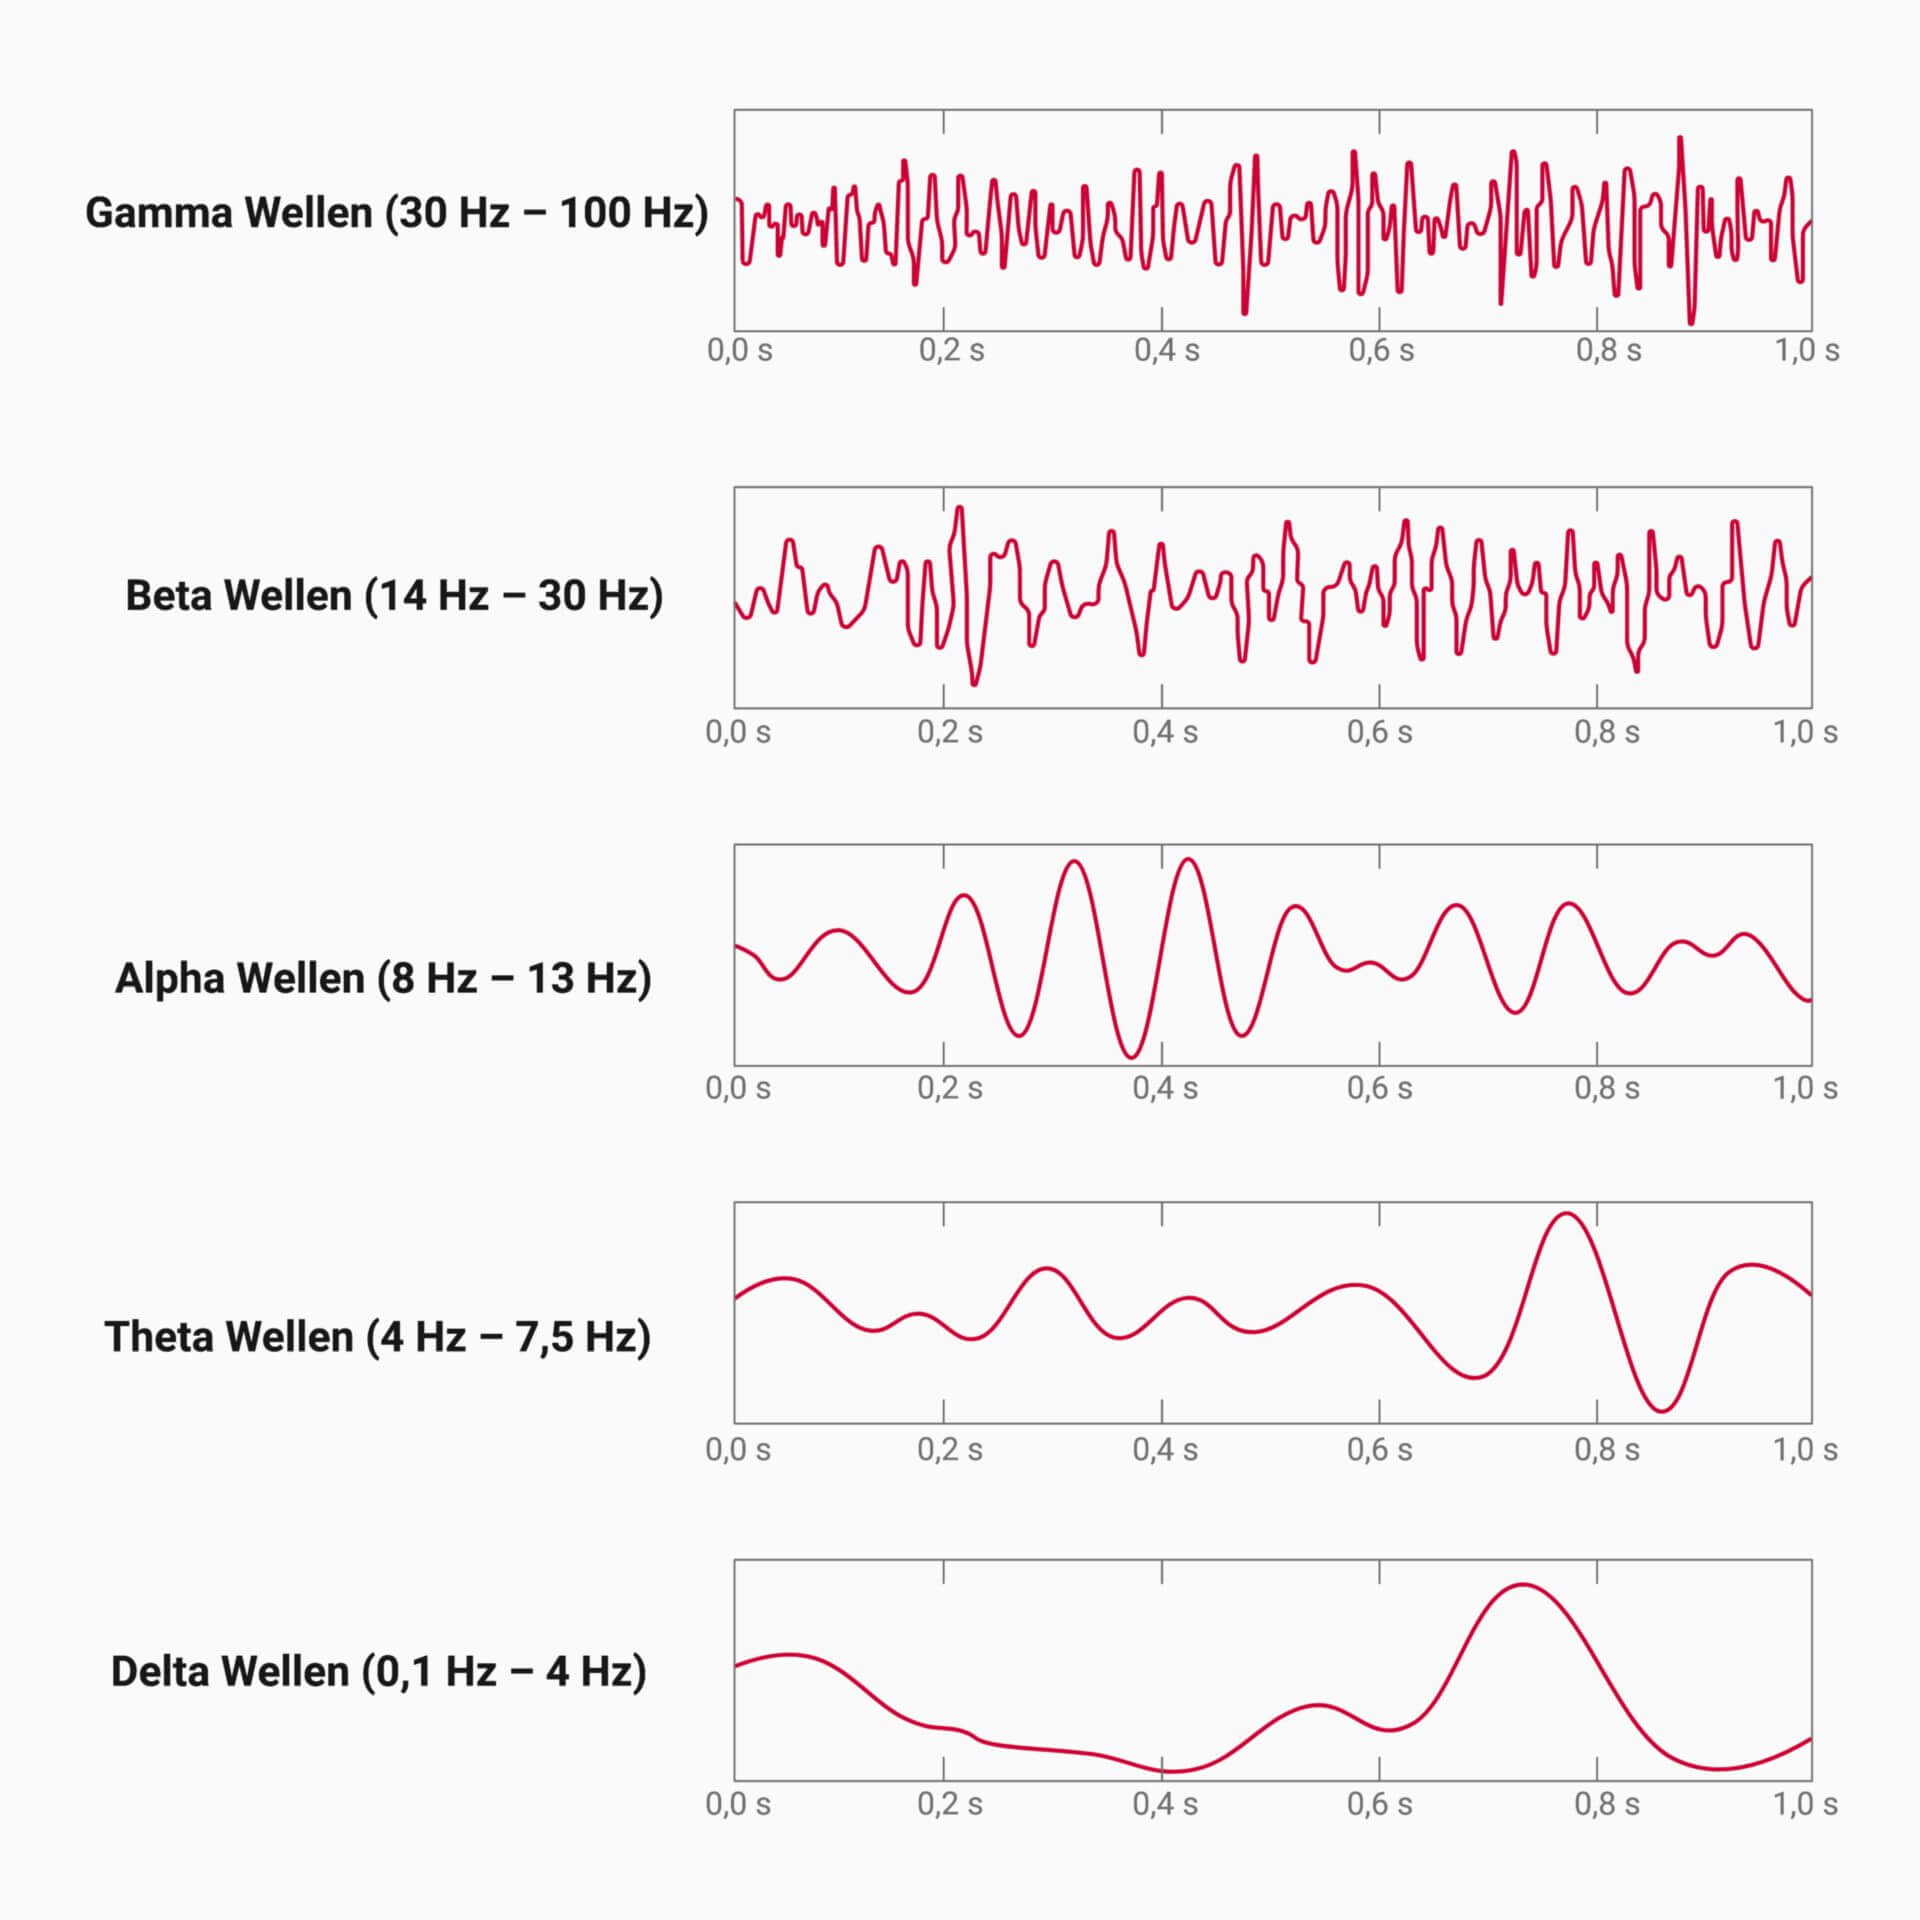
\includegraphics[width=\textwidth]{eeg-baender_lg.jpg}
        \caption{Übersicht EEG-Signaltypen \cite{pic_eeg}}
        \label{EEG_pic}
    \end{subfigure}
    \hfill
    \begin{subfigure}{0.45\textwidth}
        \centering
        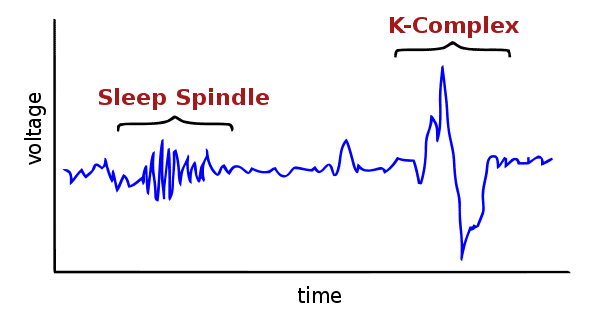
\includegraphics[width=\textwidth]{schlapfspindel_k_komplex.png}
        \caption{Schlafspindeln und K-Komplex-Gehirnströme \cite{pic_spin_k_komp}}
        \label{spind_k_pic}
    \end{subfigure}
    \caption{EEG Signale}
\end{figure}

Die Phasen des Schlafs unterteilen sich in zwei Hauptphasen, dem Non-REM-Schlaf (NREM) und dem REM-Schlaf (Rapid Eye Movement). Während des Schlafens ändern sich die Hirnströme, was mittels Elektroenzephalographie (EEG) zu erfassen ist. Das EEG misst die Potentialveränderung des Gehirns, welche die elektrische Aktivität des Gehirns darstellt und grafisch darstellbar ist, wie in Abbildung (\ref{EEG_pic}) erkennbar. Die Abbildung zeigt beispielhaft verschiedene Frequenzbänder (EEG-Bänder). Ganz grob lassen sich die Bänder-Ausschläge beurteilen, wenn es nach unten ausschlägt, eine Positivierung, sind die tiefen Schichten erregt (erregendes postsynaptisches Potential) oder die oberflächlichen Schichten inhibiert (inhibitorisches postsynaptisches Potential), entsprechend beim ein Ausschlag nach oben, einer Negativierung, vice versa.  \cite{flexikon}

Der NREM lässt sich in drei Stadien unterteilen (N1-N3), dazu noch die REM-Phase und der Wachzustand:
\begin{itemize}

\item \textbf{Wachphase}\\
Im EEG sind zunächst \(\beta\)-Wellen zu erkennen Abb.\ref{EEG_pic}, je schläfriger die Person wird, desto dominanter werden die \(\alpha\)-Wellen.

\item \textbf{Stage 1: N1 - leichter Schlaf}\\
Macht 5 \% der Schlafzeit aus und dauert ca. 1 - 5 Minuten. Es ist die Übergangsphase von wach zu schlafend. Das EEG zeigt \(\theta \)-Wellen Abb.\ref{EEG_pic} (niedrige Spannung), diese Phase beginnt, wenn mehr als 5ß\% der \(\alpha\)-Wellen durch niederfrequente Wellen ersetzt wurden. Diese Phase ist die Übergangsphase und soll den Körper auf tiefere Schlafphasen vorbereiten.

\item \textbf{Stage 2: N2 - tieferer Schlaf}\\
Die Dauer dieser Phase beginnt im ersten Schlafzyklus mit ~25min und wird im Verlauf der Nacht länger, sie macht 45\% der Schlafzeit aus. Das EEG zeigt K-Komplexe und Schlafspindeln, siehe Abbildung (\ref{spind_k_pic}). K-Komplexe sind biphasische Wellen hoher Amplitude (~125-150\(\mu\)V) und niedriger Frequenz(1-2Hz). K-Komplexe werden durch akustische Reize provoziert, sie spiegeln die Wahrnehmung von Umweltreizen wieder. Schlafspindeln haben eine hohe Frequenz (11-15Hz) und eine niedrige Amplitude (<50\(\mu\)V), man nimmt einen schlafstabilisierenden Effekt an, da sie aus hemmenden Rückkopplungen der Nervenfasern entstehen, die vom Thalamus zur Großhirnrinde gehen. Die Schlafspindeln sind kennzeichnend für Schlaf. \cite{flexikon} \cite{pschyrembel_267}

In dieser Phase beginnt der Körper sich zu entspannen, Herzfrequenz und Körperthemperatur sinken.

\item \textbf{Stage 3: N3 - tiefster, NREM Schlaf}\\
Wird auch slow-wave-sleep (SWS) genannt und beansprucht etwa 25\% der Schlafzeit. Im EEG sind \(\delta\)-Wellen erkennbar Abb.\ref{EEG_pic}, diese haben die niedrigste Frequenz und die höchste Amplitude. N3 ist eine sehr tiefe Schlafphase mit einer hohen Weckschwelle und ist essenziell für die systemische Regeneration des Körpers. Das beinhaltet die Reparatur und das Wachstum von Geweben und Stärkung des Immunsystems.

\item \textbf{REM Schlaf}\\
Die Dauer der REM-Phase umfasst 25\% der Schlafzeit, beginnt etwa 90min nach dem Einschlafen mit ~10min Dauer und wird mit jedem Schlafzyklus länger, sie kann bis zu 1h dauern. Kennzeichnend für diese Phase ist die schnelle, unregelmäßige Bewegung der Augen, auch rapid eye movement. Die Skelettmuskulatur ist fast völlig erschlafft, während diee Gehirnaktivität, der Blutdruck und die herz- und Atemfrequenz erhöht sind. Das EEG zeigt vorallem \(\beta\)-Wellen Abb.\ref{EEG_pic}, diese liegen bei 14-30Hz. \(\beta\)-Wellen treten neben der REM Phase bei wachen Personen auf, deren Kortex (Hirnrinde) gerade am Arbeiten ist. Im REM-Schlaf sollen sich Gedächtnisinhalte festigen. \cite{flexikon}

\end{itemize}

Ein Schlafzyklus läuft in der Reihenfolge N1 - N2 - N3 - REM ab und dauert ~90-110min. In dem ersten Zyklus ist die REM-Phase noch kurz, aber wird mit jedem Zyklus zum Morgen hin länger.  \cite{phys_sleep_stages}

\subsubsection{Pathophysiologie Schlafapnoe}\label{schlafapnoe}
Die obstruktive Schlafapnoe (OSA) gehört zu den schlafbezogenen Atmungsstörungen (SBAS) und ist eine Erkrankung die durch wiederholte Atempausen während des Schlafens gekennzeichnet ist. Es gibt vier verschiedene Phänotypen die eine OSA verursachen können:

5.1 Obstruktive Schlafapnoe
Entsprechend der ICSD-3 [10] wird eine
obstruktive Schlafapnoe (OSA) dann diagnostiziert, wenn die Atmungsstörung
durch keine andere Schlafstörung oder
medizinische Erkrankung oder durch
Medikamente oder andere Substanzen
erklärbar ist und entweder ein AHI >
15/h (Ereignis jeweils größergleich 10 s) Schlafzeit oder ein AHI größergleich 5/h Schlafzeit in
Kombination mit einer typischen klinischen Symptomatik oder relevanten
Komorbidität vorliegt. 
Tagesschläfrigkeit bis hin zum unfreiwilligen Einschlafen ist das führende klinische Symptom der obstruktiven Schlafapnoe --Hauptbefund
Nächtliches Aufschrecken mit kurzzeitiger Atemnot, Schnarchen (bei 95prozent der Betroffenen),  Isoliert betrachtet, weisen die Symptome jedoch nur eine geringe Spezifität auf  --Nebenbefund
--> Definition OSA

\begin{itemize}
\item \textbf{Anatomische Einschränkungen der oberen Atemwege:}\\
Hierbei handelt es sich um strukturelle Faktoren, wie eine Verengung der Atemwege durch vergrößerte Mandeln, Fettansammlungen oder andere anatomische Besonderheiten. Diese Phänotypen sind häufig bei übergewichtigen oder älteren Menschen zu beobachten.

\item \textbf{niedrige respiratorische Erregungsschwelle (Arousals):}\\
Eine niedrige Erregungsschwelle bedeutet, dass Personen während des Schlafs leichter durch Atemprobleme geweckt werden. Dies führt zu fragmentiertem Schlaf und verhindert eine kontinuierliche Atmung. Umgekehrt kann eine zu hohe Schwelle die Sauerstoffsättigung gefährlich abfallen lassen.

\item \textbf{Instabilität des Atemantriebs („Loop Gain“):}\\
Diese Phänotypen beschreiben Menschen, deren Atmungssystem zu Überreaktionen neigt, was zu wechselnden Phasen von Hyperventilation und Hypoventilation führt. Dies verstärkt das Auftreten von Atempausen und Sauerstoffmangel.

\item \textbf{schlechte Funktion der oberen Atemwegsmuskulatur:}\\
Hier liegt das Problem in einer unzureichenden Aktivierung oder Kontrolle der Muskeln, die die Atemwege während des Schlafs offenhalten sollten. Besonders während des REM-Schlafs, in dem der Muskeltonus generell abnimmt, kann dies zu Atemwegsblockaden führen.
\end{itemize}
Diese Phänotypen sind nicht immer isoliert, sondern treten oft in Kombination auf. Ein besseres Verständnis der individuellen Merkmale ermöglicht eine gezieltere Diagnostik und Therapie der OSA. So können gezielte Therapielösungen für die spezifischen Pathomechanismen entwickelt werden. 
\cite{OSA_Pathophysiology2019} \cite{DGSM2017}

\subsubsection{Therapie Schlafapnoe}\label{therapy}

Die Behandlung der obstruktiven Schlafapnoe (OSA) richtet sich nach dem individuellen Beschwerdebild, den Begleiterkrankungen sowie den persönlichen Bedürfnissen und dem Therapiewillen des Patienten. Ziel ist es, die schlafbezogenen Atmungsstörungen zu beseitigen, die Schlafqualität zu verbessern und das Risiko für kardiovaskuläre und andere Komplikationen zu senken. Abhängig von der Schwere der Erkrankung stehen verschiedene Therapieansätze zur Verfügung, die von konservativen Maßnahmen über apparative Unterstützung bis hin zu chirurgischen Eingriffen reichen. \cite{DAE81892} \cite{flexikon}

\begin{itemize}
    \item \textbf{apparative Therapie}\\
    Die Standardtherapie der obstruktiven Schlafapnoe ist die nächtliche Überdruckbeatmung („positive airway pressure“, PAP), als die konkrete Referenzmethode im kontinuierlichen PAP-Modus (CPAP, „continuous positive airway pressure“). Die Indikationsstellung zur CPAP-Therapie erfolgt anhand einer Kombination aus klinischer Anamnese, polysomnographischem Befund und Begleiterkrankungen. Besonders wenn ohne Therapie eine Verschlechterung dieser Erkrankungen zu erwarten ist, wird eine CPAP-Therapie empfohlen. Der Therapiewille des Patienten sowie dessen individuelle Situation spielen ebenfalls eine entscheidende Rolle.
    
    Neben CPAP kommt auch der APAP-Modus (automatisch titrierendes PAP) zum Einsatz, der den Atemwegsdruck flexibel an die Bedürfnisse des Patienten anpasst. Beide Ansätze zielen darauf ab, den Kollaps der oberen Atemwege zu verhindern und die Atmung während des Schlafes zu stabilisieren. Kontraindikation der APAP sind zentrale Atmungsstörungen, kardio- pulmonale Erkrankungen und nächtliche Hypoventilationen. Die APAP kommt vorallem zum Einsatz bei Patienten, die den kontinuierlichen Druck der CPAP nicht mehr ertragen, bei komplexen Apnoen oder mangelnder Compliance. 

    \item \textbf{konservative Therapie}\\
    Konservative Maßnahmen umfassen Lebensstiländerungen wie Gewichtsreduktion, die Vermeidung von Alkohol und Sedativa sowie das Einhalten einer guten Schlafhygiene. Bei lageabhängiger OSA kann Lagetraining, das eine Rückenlage vermeidet, ebenfalls hilfreich sein.

    \item \textbf{medikamentöse Therapie}\\
    Medikamentöse Ansätze spielen bei der Behandlung der OSA nur eine untergeordnete Rolle, da bisher keine Substanzen eine ausreichende Wirksamkeit gezeigt haben.

    \item \textbf{chirurgische Therapie}\\
    Operative Eingriffe werden nur bei spezifischen anatomischen Ursachen wie Tonsillenhyperplasie oder kraniofazialen Fehlbildungen in Betracht gezogen. Zu den Methoden zählen beispielsweise die Uvulopalatopharyngoplastik oder Kieferrekonstruktionen. 
    
    Die Uvulopalatopharyngoplastik mit Tonsillektomie nach Fujita, die TE-UPPP, ist ein chirurgisches Verfahren bei welchem die Atemwege durch Entfernung von überschüssigem Gewebe erweitert werden. Das Ziel des Eingriffs ist eine Verringerung der Kollapsneigung der oberen Atemwege während des Schlafens. Im Rahmen eines Case Reports war eine Indikation der OSA einen verengten oropharyngealen Raum mit vergleichsweise großer Uvula (Gaumenzäpfchen) und überschüssiger Mucosa (Schleimhaut) des umgebenden Gewebes. Die Tonsillektomie ist die vollständige chirurgische Entfernung der Tonsilla Palatina (Gaumenmandel). Anschließend wird redundante Mucosa entfernt und das Uvula korrigiert. \cite{Fujita_UPPP}
\end{itemize}

\newpage
\subsubsection{prisma Smart} % Text ausbauen!
Das prisma SMART ist ein druckkontrolliertes, nicht-invasives Therapiegerät, das zur Behandlung schlafbezogener Atmungsstörungen (SBAS) wie der obstruktiven Schlafapnoe (OSA) mit Maske eingesetzt wird (Kapitel \ref{schlafapnoe}). Es nutzt den autoCPAP-Modus, der den Therapiedruck kontinuierlich anpasst, um die oberen Atemwege des Patienten offen zu halten und so Atemaussetzer während des Schlafes zu verhindern. Dieser Modus ist besonders effektiv bei der Behandlung der OSA, da er den Druck anpasst, um die Atemwege während des gesamten Schlafzyklus offen zu halten. Im Vergleich zu anderen Geräten wie dem CPAP-Modus, der einen konstanten Druck liefert, bietet der autoCPAP-Modus eine individuellere Anpassung (Kapitel \ref{therapy}). 

Die physiologische Grundlage dieser Therapie beruht auf der Pathophysiologie der OSA, bei der es zu wiederholten Atempausen aufgrund eines Kollapses der oberen Atemwege kommt. Während des Schlafs, insbesondere in der REM-Phase, verringert sich der Muskeltonus, was das Risiko von Atemwegsverengungen erhöht. Der prisma SMART wirkt dem entgegen, indem er durch den erzeugten Überdruck die Atemwege stabilisiert, was die nächtlichen Atemaussetzer verhindert und eine ausreichende Sauerstoffversorgung sicherstellt. Dies fördert nicht nur die Atmung, sondern verbessert auch die Schlafqualität.
\cite{manual_smart}

\begin{figure}
	\centering
	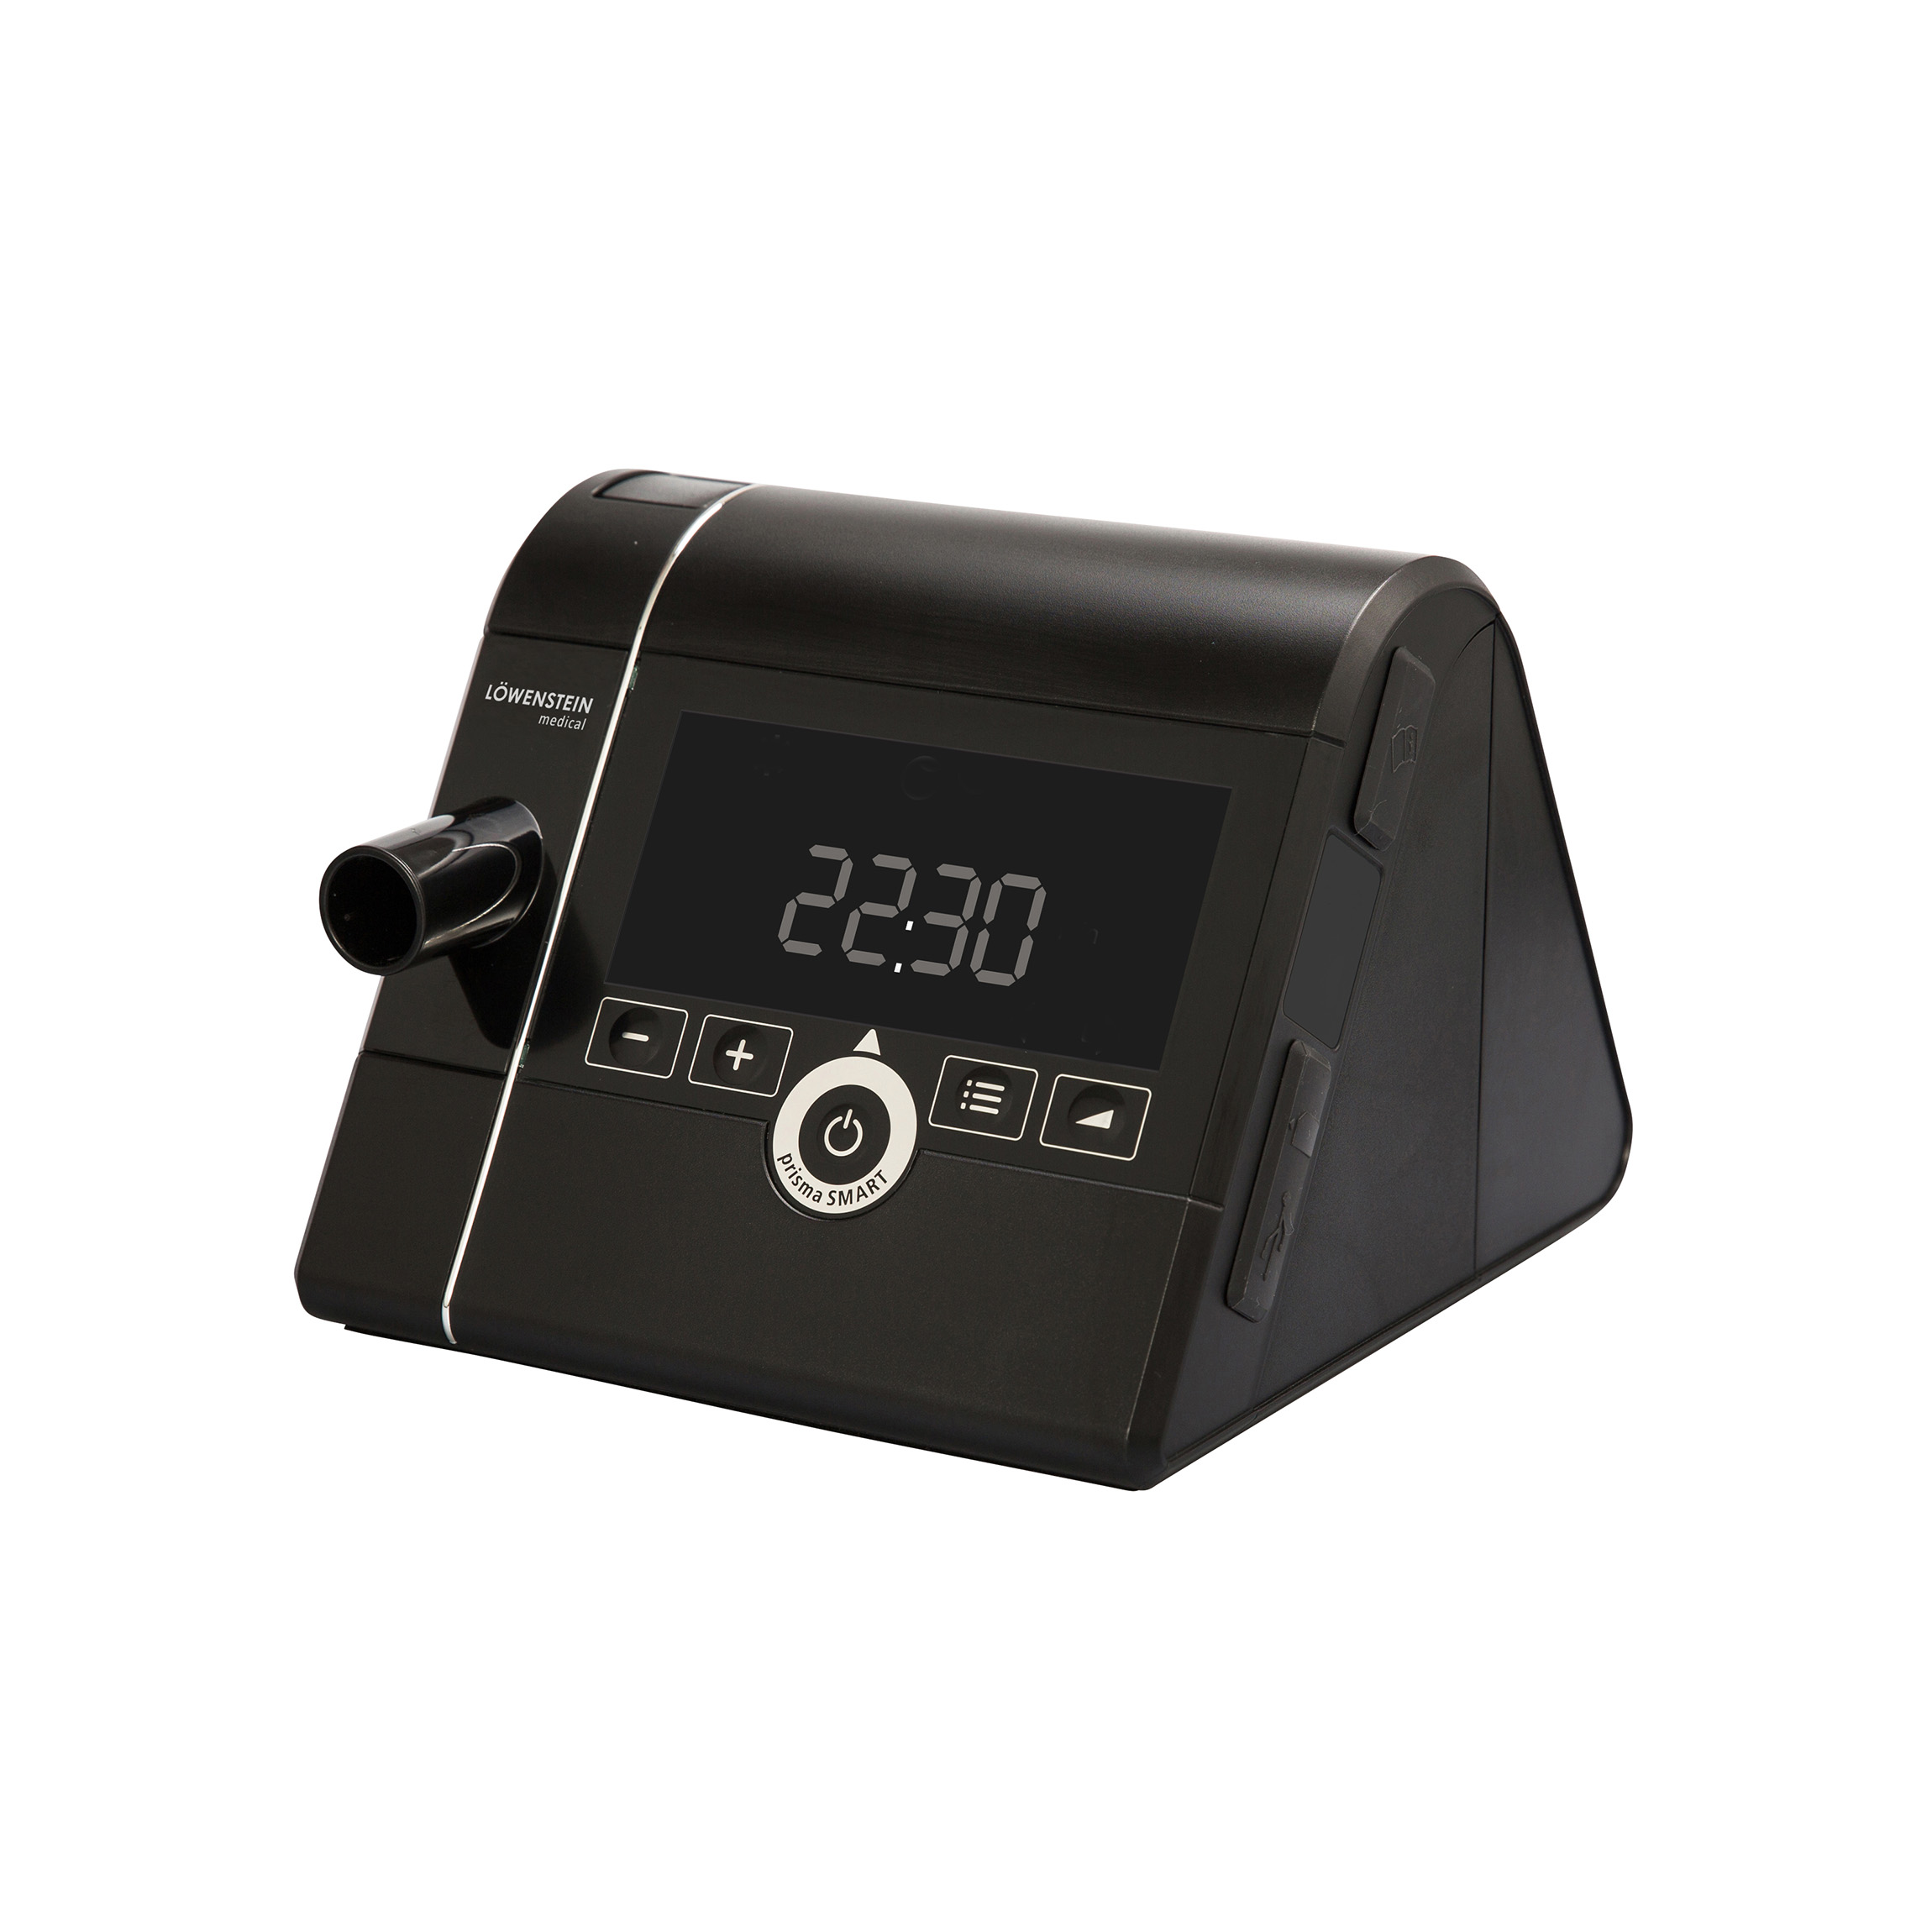
\includegraphics[width=0.45\textwidth]{prisma_SMART.jpg}
	\caption{prisma SMART \cite{pic_prisma_smart}}
	\label{pic_prismaSMART}
\end{figure}

\newpage
\subsection{Qualitätsmanagement}\label{Qualitätsmanagement}
MDR, IVDR, AIMDD, etc

\subsection{Meetings}\label{Meetings}
SCRUM - Erklären
% wichtig - LM macht es nicht ganz nach Vorschrift, klassische Strukturen auch drin
\\ 
\textbf{SCRUM}\\
Scrum ist ein systematischer Ansatz um Projekte strukturiert durchzuführen. Es soll die Teams bei der Lösung komplexer Probleme unterstützen indem Rollen, Regeln und Ereignisse definiert werden. Die zugrundeliegenden Prinzipien sind Empirie und Lean Thinking. 
„Empirie, die Erfahrung selbst und die auf Erfahrung beruhende Erkenntnis.  
 \cite{dorsch_empirie}" 

something something 
\cite{scrum2020}

\newpage
\section{Aufgaben}\label{Aufgaben}
In diesem Abschnitt werden die Tätigkeiten während des Praxissemesters im Überblick dargestellt. Aufgrund der Vertraulichkeit und der wirtschaftlichen Sensibilität der zugrunde liegenden Daten ist eine detaillierte Darstellung spezifischer Inhalte nur eingeschränkt möglich.

\subsection{Dokumentationsautomatisierung}\label{Dokumentationsautomatisierung}
In der Softwareentwicklung ist das Testen essenziell, um die Funktionalität und Korrektheit des Codes sicherzustellen. Ein entscheidender Aspekt dabei ist die Dokumentation der durchgeführten Tests, einschließlich verwendeter Parameter und spezifischer Bedingungen. Dieser Prozess kann zeitintensiv sein. \\
Um diesen Aufwand in Zukunft zu minimieren, wird ein Tool entwickelt, das während der Testlaufzeit automatisch die benötigte Dokumentation erstellt und diese direkt in das entsprechende Workitem auf Polarion hochlädt.

\subsubsection{Polarion}\label{polarion}
Polarion (Siemens Company) ist eine webbasierte Anforderungsmanagement-Software, die Unternehmen dabei unterstützt, den gesamten Lebenszyklus von Projekten und Produkten effizient zu verwalten. Als integrierte Lösung bietet Polarion eine Plattform, auf der Anforderungen, Tests, Fehler und Änderungsanfragen nahtlos miteinander verknüpft werden können.

Die Software basiert auf drei Kernprinzipien: Zusammenarbeit (Collaboration), Rückverfolgbarkeit (Traceability) und Workflow-Management. Diese Prinzipien ermöglichen es Teams, in Echtzeit zu kommunizieren und Projekte durchgängig transparent und nachvollziehbar zu gestalten.

Polarion zeichnet sich durch folgende Funktionen aus:\\
\textbf{Webbasierter Zugang:} Polarion ist vollständig browserbasiert, was den Zugriff auf Projektdaten von überall ermöglicht.\\
\textbf{Rückverfolgbarkeit und Auditierung:} Jede Änderung an Anforderungen oder anderen Work Items wird automatisch versioniert und dokumentiert, was die Einhaltung von Compliance- und Auditvorgaben erleichtert.\\
\textbf{Workflow-Steuerung:} Workflows können individuell definiert werden, um sicherzustellen, dass Anforderungen und andere Objekte einen strukturierten Lebenszyklus durchlaufen.\\
\textbf{Kollaborationswerkzeuge:} Funktionen wie Wikis, Benachrichtigungen und Diskussionsforen fördern die Zusammenarbeit zwischen verschiedenen Stakeholdern, von Analysten über Entwickler bis hin zu QA-Teams.\\
Ein besonderes Merkmal von Polarion ist die Unterstützung verschiedener Entwicklungsansätze wie agiler Methoden, Wasserfall-Modellen oder hybriden Ansätzen. Teams können ihre bevorzugte Methodik nutzen und gleichzeitig von automatisierter Rückverfolgbarkeit, Versionierung und einem flexiblen Berichtswesen profitieren.

Darüber hinaus bietet Polarion die Möglichkeit, Anforderungen und Testfälle parallel zu verwalten. Mit der LiveDocs-Funktion können Teams gemeinsam an Spezifikationen arbeiten, wobei jede Änderung sofort nachverfolgbar ist. Dies erhöht die Transparenz und ermöglicht es, Anforderungen und Tests kontinuierlich abzustimmen.

Zusammenfassend unterstützt Polarion Unternehmen dabei, Projekte effizient zu planen, durchzuführen und zu dokumentieren, während gleichzeitig regulatorische Vorgaben eingehalten werden. \cite{polarion_web}


\subsubsection{Regular Expression}\label{regularExpression}
Die re-Bibliothek in Python ermöglicht die Anwendung regulärer Ausdrücke (regular expression - regex) zur flexiblen und effizienten Textverarbeitung. Regex sind Muster, die gezielt nach Zeichenfolgen in Textdaten suchen und so vielfältige Datenoperationen ermöglichen. Mit der re-library können Funktionen wie search, match, findall und sub genutzt werden, um beispielsweise Texte zu durchsuchen, Muster zu ersetzen und Daten zu validieren. \cite{regex_lib}

Die wichtigsten Funktionen der Bibliothek sind:
\begin{itemize}
    \item \texttt{search()} – sucht das erste Vorkommen eines Musters im Text.
    \item \texttt{match()} – prüft, ob der Text mit dem Muster beginnt.
    \item \texttt{findall()} – gibt alle Vorkommen des Musters als Liste zurück.
    \item \texttt{sub()} – ersetzt alle Vorkommen des Musters durch einen angegebenen String.
\end{itemize}

\newpage
Die re-Syntax bietet eine Vielzahl von Operatoren zum definieren der Muster:
\begin{table}[h!]
\centering
\begin{tabular}{|c | >{\arraybackslash}p{11cm}|}
\hline
\texttt{.} & steht für ein beliebiges Zeichen (außer Zeilenumbrüche) \\
\hline
\texttt{\textbackslash} & danach kommt ein Charakter mit vordefinierter Funktion zB \texttt{\textbackslash d}  matched
	alle Unicode decimal Ziffern \\
\hline
\texttt{* +} & geben null oder mehr (\texttt{*}) bzw. mindestens 
	eine (\texttt{+}) Wiederholungen des vorherigen Elements an. \\
\hline
\texttt{[] ()} & definiert Zeichenmengen (\textit{sets}), zB \texttt{[abc]} für die Zeichen 	 
	\texttt{a}, \texttt{b} oder \texttt{c}. \\
\hline
\end{tabular}
\end{table}

\begin{lstlisting}[language=Python, caption=Beispiel für Python-Code]
import re

txt = "Das ist ein string mit 123 Zahlen"
pattern = r"\d+" # alle Ziffern

# in txt wird das pattern mit "00" ersetzt
new_txt = re.sub(pattern, "00", txt)
# new_txt: Das ist ein string mit 00 Zahlen
\end{lstlisting} % code works

\subsection{Library Adapter}\label{LibraryAdapter}
Eine Library durch eine aktuellere austauschen in C++

\subsubsection{MsgPack}\label{msgpack}
library MsgPack
msgpack VS json - Vorteile
joa, hat dann die Ansprüche doch nicht erfüllt *sad trumpet*

\newpage
\section{Ergebnisse}
Präsentiere und diskutiere hier die Ergebnisse deines Berichts.

\newpage
\section{Fazit}
Im Fazit fasst du alles zusammen und gibst einen Ausblick.

\newpage
\bibliographystyle{unsrt}
\bibliography{Praxissemesterbericht_bibliographie}

\end{document}
